\documentclass{article}
\usepackage{verbatim}
\usepackage[MeX]{polski}
\usepackage[utf8]{inputenc}
\usepackage{mathtools}

\usepackage{float}

\newcommand{\tab}[1]{\hspace{.05\textwidth}\rlap{#1}}

\author{Piotr Izert, Łukasz Dragan}
\title{Algorytmy Zaawansowane - POLE}

\begin{document}

\maketitle

\newpage
\tableofcontents
\newpage


\section{Przedstawienie problemu}

\subsection{Treść zadania}
\paragraph{}\textit{
Zaprojektować i zaimplementować algorytm, który w czasie liniowym względem n oblicza pole n-wierzchołkowego prostego wielokąta oraz sprawdza, czy podany punkt leży wewnątrz tego wielokąta. Program powinien zawierać procedurę sprawdzającą, czy dany wielokąt jest prosty.
}



\section{Opis rozwiązania}

\subsection{Pole wielokąta}

\paragraph{}
W celu obliczenia pola powierzchni wielokąta prostego stosujemy algorytm wykorzystujący tzw. wzór trapezowy Gaussa \(S=\frac{1}{2}\sum\limits_{i=1}^n (x_i+x_{i+1})*(y_{i+1}-y_i)\), gdzie \(S\) to pole powierzchni wielokąta, \(x_i, y_i\ dla\ i=1...n\) to współrzędne kolejnych wierzchołków wielokąta, a \(n\) to liczba wierzchołków wielokąta. Zakładamy, że \(x_{n+1} = x_1\) oraz \(y_{n+1} = y_1\).

\paragraph{Algorytm}
%\mbox{}\\
%\(A=(x_1, y_1),..., (x_n, y_n), (x_1,y_1)\) - ciąg wierzchołków wielokąta z dodanym na koniec pierwszym wierzchołkiem.
\begin{enumerate}
\item \(area = 0\)
\item \(j=n\)
\item dla \(i=1\) do \(n\) wykonaj: %dla każdego elementu \((x_i,y_i)\) z \(A\) wykonaj:
\item \tab{\(area = area + (x_j+x_i)*(y_j-y_i)\)}
\item \tab{\(j=i\)}
\item \(area = |area/2|\)
\item RETURN \(area\)
\end{enumerate}

\paragraph{Interpretacja geometryczna} \mbox{}\\
Sumę we wzorze na pole wielokąta można interpretować jako sumę pól trapezów, z których niektóre pola wzięte są ze znakiem dodatnim, a inne z ujemnym. Zostało to zilustrowane na rysunku \ref{fig:trapez}.

\begin{figure}[H]
    \centering
    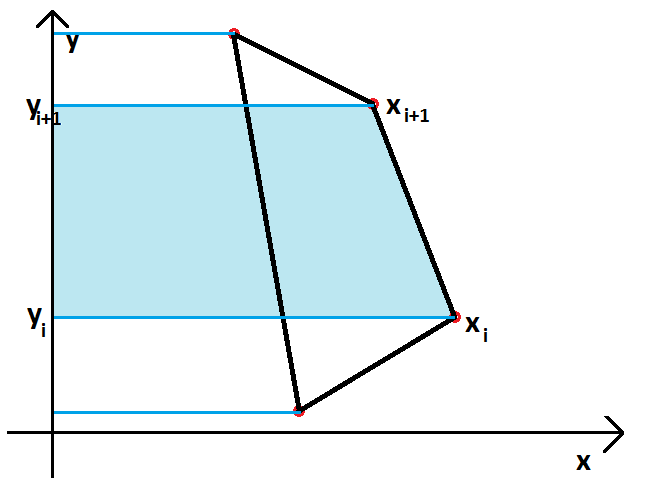
\includegraphics[width=10cm]{trapez.png}
    \caption{Interpretacja geometryczna wzoru Gaussa na pole wielokąta}
    \label{fig:trapez}
\end{figure}

\subsection{Zawieranie punktu w wielokącie}

\paragraph{}
Sprawdzenie, czy punkt zawiera się w wielokącie jest realizowane przez zliczenie przecięć półprostej zaczynającej się w badanym punkcie z bokami wielokąta. Jeżeli liczba przecięć jest nieparzysta, to znaczy, że punkt leży wewnątrz wielokąta. W przeciwnym razie punkt leży na zewnątrz wielokąta.


W zaimplementowanym algorytmie półprosta prowadzona jest równolegle do osi X w kierunku rosnących wartości. Oznaczmy przez \(x_i, y_i\ dla\ i=1...n\) współrzędne kolejnych wierzchołków wielokąta, a przez \(X\) i \(Y\) współrzędne badanego punktu.

\paragraph{Algorytm}
\begin{enumerate}
\item inside = false
\item dla \(i=1\) do \(n\) wykonaj: 
\item \tab \tab sprawdź, czy krawędź \(i, i+1\) przecina prostą \(y=Y\)
\item \tab \tab jeżeli tak, to sprawdź, czy współrzędna x punktu przecięcia jest większa od \(X\)
\item \tab \tab jeżeli tak, to inside = !inside
\end{enumerate}

Sprawdzenie z punktu 3. realizowane jest w następujący sposób - sprawdzane jest, czy współrzędne \(y\) obydwu końców krawędzi leżą na różnych półpłaszczyznach wyznaczanych przez prostą \(y=Y\) - warunek:

$$(y_i > Y) != (y_{i+1} > Y)$$

Sprawdzenie z punktu 4. realizowane jest przez znalezienie punktu przecięcia krawędzi z prostą \(y=Y\) i porównanie go do wartości \(X\):

$$X < x_i + (x_j - x_i)\frac{y_i - Y}{y_i - y_j}$$

Przykład zasady obliczania punktu przecięcia został przedstawiony na rysunku \ref{fig:przeciecie}.

\begin{figure}[H]
    \centering
    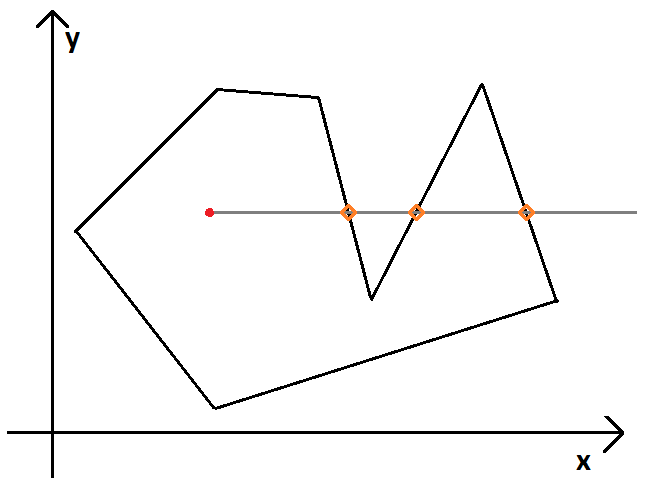
\includegraphics[width=10cm]{zawieranie.png}
    \caption{Sprawdzanie zawierania się punktu w wielokącie}
    \label{fig:zawieranie}
\end{figure}

\begin{figure}[H]
    \centering
    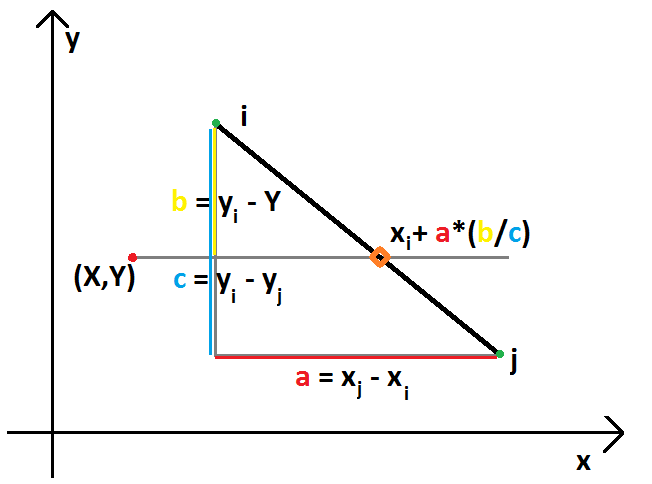
\includegraphics[width=10cm]{przeciecie.png}
    \caption{Obliczanie punktu przecięcia krawędzi z prostą}
    \label{fig:przeciecie}
\end{figure}

\subsection{Sprawdzanie, czy wielokąt jest prosty}
\paragraph{}Algorytmy prezentowane w niniejszym opracowaniu mają zastosowanie jedynie, gdy dany wielokąt jest prosty.
\paragraph{Wielokąt prosty:} wielokąt, którego boki tworzą zamkniętą łamaną, a dwa jego boki mają punkt wspólny tylko, gdy są sąsiadami. (Wikipedia)
\paragraph{Algorytm}\mbox{}\\
Sprawdzenie, czy wielokąt jest prosty odbywa się przy użyciu algorytmu Shamosa - Hoeya, który jest odmianą algorytmu znajdywania wszystkich punktów przecięcia zbioru odcinków - algorytmu Bentleya - Ottmanna. Pomysł na algorytm opiera się na scanlinii przecinającej odcinki wielokąta. Scanlinia "porusza się" wzdłuż osi $x$, jest równoległa do osi $y$ i utrzymuje kolejność punktów przecięcia ze wszystkimi aktualnie przecinanymi odcinkami posortowaną po współczędnej $y$. Przecięcia sprawdzane są tylko wśród par boków leżących obok siebie na scanlinii, dzięki czemu liczba sprawdzeń jest minimalna. Można zauważyć, że kolejność odcinków na scanlinii może zmieniać się tylko, gdy scanlinia mija początek odcinka (dodanie odcinka), koniec odcinka (usunięcie odcinka) lub przecięcie odcinków (zamiana odcinków miejscami). W tym przypadku nie trzeba rozważać przecięcia, bo znalezienie jakiegokolwiek przecięcia kończy działanie algorytmu (oznacza, że wielokąt nie jest prosty). Schemat działania algorytmu:
\begin{enumerate}
    \item Zainicjalizuj kolejkę zdarzeń. Zdarzeniem dla scanlinii jest napotkanie początku lub końca odcinka, w zdarzeniu należy więc zapisać jego typ (początek lub koniec krawędzi) oraz której krawędzi dotyczy. Zdarzenia w kolejce są posortowane według punktów, w których zachodzą, rosnąco względem współrzędnej $x$, w przypadku równości rosnąco względem współrzędnej $y$.
    
    \item Zainicjalizuj scanlinię jako pustą
    
    \item Dla każdego zdarzenia z kolejki:
    
    \item \tab jeśli jest to początek krawędzi, dodaj krawędź do scanlinii i sprawdź, czy przecina się ona ze swoimi sąsiadami (krawędzią bezpośrednio niżej i wyżej na scanlinii), jeśli tak, return $FALSE$
    
    \item \tab jeśli jest to koniec krawędzi, to usuń krawędź ze scanlinii, i sprawdź, czy jej wcześniejsi sąsiedzi przecinają się, jeśli tak, return $FALSE$
    
    \item return $TRUE$
\end{enumerate}

Przy sprawdzaniu przecięć odcinków potrzebna jest funkcja, która zwraca położenie punktu $P_2$ względem prostej $P_0$ $P_1$. Żeby to określić, należy wyliczyć różnicę iloczynów:
$$ (P_1.x - P_0.x)*(P_2.y - P_0.y) - (P_2.x - P_0.x)*(P_1.y -  P_0.y) $$
Wynik dodatni oznacza, że $P_2$ leży na lewo od $P_0P_1$, wynik 0 oznacza, że $P_0$, $P_1$ i $P_2$ są współliniowe, natomiast wynik ujemny oznacza, że $P_2$ leży na prawo od $P_0P_1$.

Wiedząc, że punkty są współliniowe, sprawdzenie, czy $P_2$ leży na odcinku $P_0P_1$ można zrealizować przez sprawdzenie, czy wartości współrzędnych $x$ i $y$ punktu $P_2$ zawierają się między wartościami odpowiednich współrzędnych punktów $P_0$ i $P_1$. 

Sprawdzanie przecięć pomięcdzy parą odcinków odbywa się wg. następującego algorytmu:

\begin{itemize}
    \item Jeżeli są to sąsiednie odcinki, to sprawdź, czy się nakładają - czy początek odcinka 1, punkt wspólny odcinków i koniec odcinka 2 są współliniowe, a koniec odcinka 2 leży na odcinku 1 lub koniec odcinka 1 leży na odcinku 2 (wg algorytmów podanych wyżej). Jeżeli się nakładają, to wielokąt nie jest prosty.
    \item W przeciwnym przypadku sprawdź przecinanie się odcinków - czy początek i koniec odcinka 1 leżą po przeciwnych stronach prostej wyznaczanej przez odcinek 2 i czy początek i koniec odcinka 2 leżą po przeciwnych stronach prostej wyznaczanej przez odcinek 1 (wg algorytmu powyżej). Jeżeli oba warunki zachodzą, to odcinki się przecinają i wielokąt nie jest prosty.
\end{itemize}



\section{Analiza poprawności}

\subsection{Pole wielokąta}
\paragraph{Poprawność} \mbox{}\\
W pierwszej iteracji pętli z kroku 3. \(area = (x_n+x_1)*(y_n-y_1) (=(x_n+x_{n+1})*(y_n-y_{n+1}))\). W kolejnych iteracjach \(j\) jest zawsze o \(1\) mniejsze od \(i\), stąd do \(area\) dodawana jest wartość \((x_j+x_{j+1})*(y_j-y_{j+1})\ dla\ j = 1...n-1\). Stąd ostatecznie \(area = (x_n+x_{n+1})*(y_n-y_{n+1}) + (x_1+x_2)*(y_1-y_2) + ... + (x_{n-1}+x_n)*(y_{n-1}-y_{n}) = \sum\limits_{i=1}^n (x_i+x_{i+1})*(y_{i+1}-y_i)\). Po podzieleniu \(area\) przez \(2\) i wzięciu wartości bezwzględnej otrzymujemy wzór Gaussa na pole powierzchni wielokąta.


\paragraph{Złożoność czasowa} \mbox{}\\
Algorytm działa w czasie \(O(n)\), gdyż główna pętla algorytmu wykonuje dokładnie \(n\) kroków.


\subsection{Zawieranie punktu w wielokącie}

\paragraph{Poprawność} \mbox{}\\
Każde przecięcie z krawędzą wielokąta podążając od badanego punktu wzdłuż półprostej można traktować jako zmianę położenia z \emph{wewnątrz} na \emph{na zewnątrz} wielokąta lub odwrotnie.

Jeżeli badany punkt leży na zewnątrz wielokąta, to podążając wzdłuż półprostej za każdym razem gdy znajdziemy się wewnątrz wielokąta, musi nastąpić moment wyjścia z powrotem na zewnątrz (ponieważ wielokąt ma skończone rozmiary). W związku z tym liczba przecięć z krawędziami wielokąta musi być \textbf{parzysta}.

Z kolei jeśli punkt leży wewnątrz wielokąta, to podązając wzdłuż półprostej co najmniej raz musi nastąpić wyjście na zewnątrz. Po każdym ewentualnym wejściu do wewnątrz nastąpi kolejne wyjście na zewnątrz, więc liczba przecięć półprostej z bokami wielokąta musi być \textbf{nieparzysta}.

\paragraph{Złożoność czasowa} \mbox{}\\
Algorytm wykonuje $n$ iteracji pętli (pętla po wszystkich krawędziach). W każdej iteracji sprawdzane jest przecięcie z prostą $y = Y$ (realizowane w czasie liniowym) oraz ewentualne położenie punktu przecięcia względem $X$ (również w czasie liniowym) - opisy sprawdzeń przy opisie algorytmu. W związku z tym złożoność czasowa algorytmu wynosi $O(n) * O(1) * O(1) = O(n)$.


\subsection{Sprawdzanie, czy wielokąt jest prosty}

\paragraph{Poprawność} \mbox{}\\
Algorytm sprawdza pod katem przecięć każde dwa odcinki, które znajdą się obok siebie na scanlinii. Łatwo sprawdzić, że zawsze gdy odcinki się przecinają, to bezpośrednio przed przecięciem znajdą się obok siebie na scanlinii, więc ich przecięcie będzie sprawdzone i wykryte.

\paragraph{Złożoność czasowa} \mbox{}\\
Inicjalizacja kolejki zdarzeń dla scanlinii wymaga czasu $nlog(n)$, ponieważ trzeba posortować początki i końce odcinków.

Scanlinia może zostać zaimplementowana jako zrównoważone drzewo binarne, dzięki czemu koszt operacji dodawania i usuwania do niej krawędzi jest rzędu $log(n)$. Dla każdego z $2n$ (początek i koniec boku) zdarzeń należy wykonać operację na drzewie i sprawdzenie przecięć. Sprawdzenie realizowane jest w czasie liniowym (wykonuje jedynie kilka operacji mnożenia, odejmowania i porównywania). W związku z tym algorytm działa w czasie $O(nlog(n) + 2nlog(n)) = O(nlog(n))$.

\section{Opis wejścia/wyjścia}

\subsection{Wejście}

\paragraph{}
Program domyślnie jako wejście przyjmuje zawartość pliku ,,in.txt'', który powinien zawierać w kolejnych liniach:
\begin{enumerate}
\item Dane postaci \(x_1\ y_1\ ...\ x_n\ y_n\), gdzie \((x_i,y_i) \in \Re^{2} \ dla\ i=1,2,...,n\) to współrzędne kolejnych punktów a \(n\) to liczba wierzchołków wielokąta.
\item Dane postaci \(x\ y\), gdzie \((x,y) \in \Re^{2}\) będące współrzędnymi punktu, którego zawieranie w wielokącie ma zostać sprawdzone.
\end{enumerate}

\paragraph{Przykładowe wejście} \mbox{}\\
\texttt{
344,8 91,2 68,8 121,6 352,8 218,4 448 114,4\\
288,8 136
}

\subsection{Wyjście}

\paragraph{}
Rezultat działania programu zapisywany jest w pliku ,,out.txt'' w postaci \(S\ Ans\) gdzie \(S\) to pole powierzchni wielokąta a \(Ans\in\{"TAK","NIE"\}\) to odpowiedź na pytanie, czy dany punkt jest zawarty w wielokącie. W przypadku, gdy dany wielokąt nie jest prosty, rezultatem działania programu jest \texttt{NOT SIMPLE}. Jeżeli dane podane na wejściu są niepoprawne, program zapisze do pliku \texttt{BAD INPUT}.

\paragraph{Przykładowe wyjście} \mbox{}\\
\texttt{1243,33 TAK}

\end{document}
